%{\Large  From Conceptual Spaces to Type Theory}

\subsection{Type Theoretic Foundations for Hypergraph-Based Data Sharing}



\p{Data communications is a trade-off between optimization
for space and bandwidth (often it is important to limit the number of
bytes in each unit of information to a minimum), security, and
programmability (networks that aim to support many developers spread
across multiple projects and institutions need to be more open-ended than
those centrally controlled by a single team).  Ideally, then,
each data type and data structure will be amenable to serialization in
multiple formats, which each elevate one priority or another; \XML{}
and \JSON{} are more flexible in an open-ended project, for example,
whereas binary serialization is more efficient.  Software models should
be rigorous: there should be documentation of reasonable values
for data fields, and (where applicable) their units of measurement;
preferably there should be some automated testing and/or type-checking
to ensure that these expectations are sustained.  Such specificity
allows programmers to maximize resources that in some contexts may
be restricted, such as internet bandwidth.  On the other hand,
requirements engineering should not degrade production performance, so
verification should be executed in a special run mode that can be
disabled for deployment, when necessary.  For speed optimization,
data types often fall back to types like 4-byte integers, which
express can support many more values than actually are conceptually
meaningful.  In these situations, the proper solution is not to
degrade runtime performance with smaller and/or more complex types
but to model those types as predeployment checks of some sort,
such as debug assertions testing the success of a type cast.
}

\p{Similarly, conceptual modeling needs to anticipate the diverse ways
that people express concepts.  For instance, 
someone's age is often measured in years, but
with respect to toddlers many people cite an age in weeks or months;
if age is extracted from textual input it is necessary to anticipate
phrases like \q{six weeks} or \q{six months}; potentially this should
be reflected in the types through which age is modeled.  If someone enters
a child's age as six months, it might be disorienting to see this
subsequently listed as, say, \q{zero years.}  This is an example of
how provisional assumptions about the proper type representation
of a human concept can be too simplistic, and therefore degrade User
Experience.  It also shows the benefit of a rich type system, where
types can be crafted to better model human concepts: if ages like
\q{six months} are recognized, then functions for comparing and binary
encoding ages need to be implemented accordingly.  A key role of a
type system is logically organizing functions necessary for the type
to work properly, which becomes more necessary as types acquire
greater complexity (in the form of special flags and values) to adapt
to human concepts and/or to interfacing with speech and natural language.
}

\p{The above examples show why semantic modeling can be important
to software development: semantic models are guidelines that improve
applications' robustness and correctness by simultaneously
codifying developers' and stakeholders' expectations and anticipating
concepts which end users will bring to bear on their interactions with
deployed software.  Unfortunately, there are several 
different notions of semantic models, 
with roots in distinct academic fields, that 
do not precisely overlap,
making it hard to integrate multiple semantic models into coherent,
multi-paradigms information systems.  Among semantic modeling paradigms,
we can perhaps identify three which are particularly influential:
grammars and lexical specifications for Natural Language Processing;
formal Ontologies described in formats such as \OWL{} (Web Ontology Language) and
providing semantics for data formats, query systems, and persistence
mechanisms such as \RDF{}, \SPARQL{}, and graph databases or \q{triple-stores};
and the formal semantics at the foundation of type systems and
implementations of concrete programming languages (implementations
of interpreters, compilers, and/or runtimes).
}

\p{In many modern-day
applications, all three of these paradigms will likely play a role.  For
example, in a medical setting, bioinformatic semantics and
communications are often modeled by some variation of \OWL{} and
\RDF{}; patients' natural language (e.g., in the form of clinical narratives)
is an essential part thorough health records; and application-specific
data types need to encapsulate aggregates of medical information
as communicated between applications via protocols such as
\DICOM{} (Digital Imaging and Communications in Medicine) and \HLSeven{}
(Health Level Seven International).  It is also important
to observe that document-level criteria (like
restrictions on \XML{} documents) do not provide enough
behavioral specification to address operational concerns,
especially in domains requiring complex calculations and
native code libraries (medical imaging, robotics,
\ThreeD{} graphics, image analysis, video analysis, or
simulations of physical systems).  Robust technology in
these environments demands that a given real-world concept is
modeled by behaviorally equivalent types at different points on a
network, and that a serialization format (like \XML{}) serves
merely as a conduit for typed values between network points.  
The components which send and receive typed values should 
be designed and tested for conformance to behavioral
expectations once they have a fully-formed instance of the
relevant type in running memory; this is a more rigorous
test than can be applied by checking an \XML{} document
against a Document Type Definition, for example.  It seems
fair to say the internet technology often fails this
standard, with a frequent use of \XML{} or \JSON{} as a
raw data stream that is processed as an untyped data structure
on the receiving end, rather than packaged into a type
or class whose overall behavioral properties are
well-documented.
}


\p{Expressing operational constraints through languages'
type systems and implementational mechanisms can be
difficult.  Consider the example of using a non-constant
reference parameter passed to a function so as to initialize
a value.  This design requires that the function body always
assign a proper value for that parameter and never attempt
to read its value prior to assignment.  This rather
straightforward requirement is hard to express in many
languages; in a pure-functional context the use
of non-constant reference parameters is not directly
allowed in the first place (forcing a more complex
syntax at the call site), whereas in an Object-Oriented
or procedural language there may be no distinct
type to capture a guarantee of initialization
(analogous to how a \const{} assertion guarantees
that a value is \q{not} changed).  Type systems
are often designed around optimizations which may be
useful in many contexts but which are not always realistic,
and the attempt to guide programmers toward writing
optimizable code can unnecessarily obscure code which
needs to be structured differently \mdash{} compare the
syntax for monads and strict evaluation in Haskell
against the (simpler and more transparent)
syntax for lazy evaluation, which is paradigmatically preferred.
 Conversely, expressing lazy evaluation in an Object-Oriented
language like \Cpp{} is convoluted and requires library support.
 These trends illustrate how type systems emerge from
(sometimes too abstract) mathematical theories and need
to be supplemented by semantic models that recognize
conceptual as well as mathematical formalisms.
}

\p{The consequence of this discussion in the present context 
concerns the problem of meta-modeling: the preferred 
frameworks wherein specific concrete data models may 
be developed.  Various data structures --- such as 
hierarchical trees or Semantic Web style graphs --- have 
been proposed as universal meta-modeles, with the 
idea that such representations are sufficiently 
abstract and flexible that they can accommodate any 
data-modeling requirements in a computational/digital 
environment.  This section, however, has attempted to 
identify reasons why these general-purpose data structures 
are suboptimal for data modeling at the level of 
Requirements Engineering and detailed procedural 
analysis.  In this book we claim that Hypergraphs, 
augmented by notions taken from Conceptual Space Theory, 
can provide a better meta-modeling foundation.
}


\subsection{Hypergraphs as a Meta-Model for Data Sharing}

\p{Publishers, in recent years, have begun to encourage authors to share their research data, and to incorporate \q{Data Availability} or \q{Supplemental Materials} sections as an integral part of their journal and book publications.  
Initiatives such \FAIRsharing{} or 
the Bill and Melinda Gates Foundation Guidelines for Authors
(which is part of \FAIRsharing{}) provide recommendations to help authors produce data sets that are Findable, Accessible, Interoperable, and Reusable (\FAIR{}).  Such initiatives represent a step  
toward realizing the goal of engineering a broad ecosystem of open-access 
scientific data --- an ecosystem that interconnects and 
interoperates with both 
scientific publications and scientific-computing software applications.  
However, this goal is hard to attain because, in reality, 
scientific applications, publishing 
software, and data-hosting technology remain largely 
siloed from one another.
}

\p{The \FAIRsharing{} standards also include 
several dozen domain-specific guidelines collectively 
referred to as \MIBBI{} (Minimum Information for Biological and Biomedical Investigations).  The \MIBBI{} specifications serve as a checklist 
for authors preparing data sets to ensure that they properly, 
and in sufficient detail, document their research and/or laboratory 
protocols (there are also research-documentation formats 
associated with specific publishing platforms, such as 
\textit{Springer Protocols}, part of Springer Nature).
As these examples demonstrate, researchers have numerous 
options for how they may document their research data.  However, 
none of these documentation format options are closely integrated 
either with publishing software --- in particular, with software 
used to compose books/articles for publication --- nor 
with scientific software applications used to acquire, analyze, and 
visualize research data.
}   

\p{Data-sharing in the publishing context is often based on 
the Semantic Web.  For example, \q{Research Objects} --- a standard 
model for composing reusable data sets --- relies on the canonical 
Semantic Web data format, \RDF{} (Resource Description Framework), 
to encode research meta-data.  Semantic Web data is often criticized, 
however, for being \q{flat} --- that is, \RDF{} does not directly 
recognize any information structures which involve multiple 
levels or organization, or contexts: data collections (such as unordered 
sets or ordered lists), clusters of interrelated pieces of information, 
contexts where certain connections between information units 
have elevated significance, and so forth.  To redress these 
limitations, multi-tier models such as Property Graphs and Hypergraphs 
have been proposed as alternative vehicles for Semantic Web data.  
While Property Graph and Hypergraph Database 
Engines are increasingly popular in business \IT{}, these 
technologies have not been comparably adopted within the publishing 
industry.
}  


\begin{figure}
\hspace{-2em}%
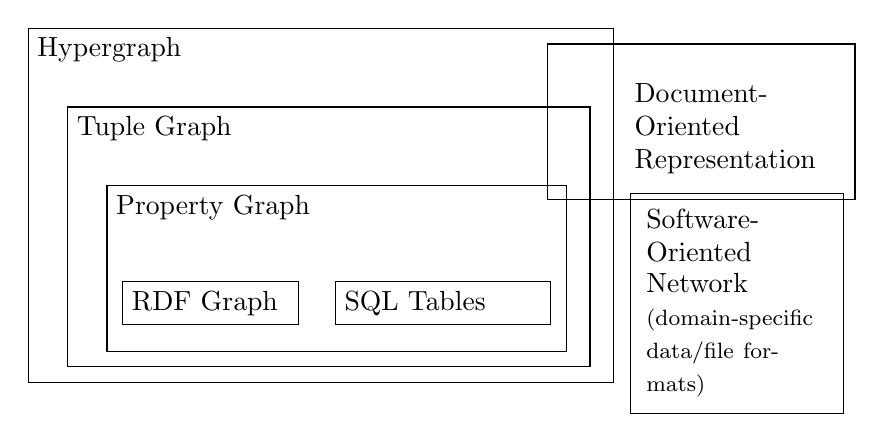
\begin{tikzpicture}
%\usetikzlibrary{shapes}
%\usetikzlibrary{positioning}
%\node[inner sep=0pt] (tbl) at (0,0)

\node [anchor=north west, text width=7.2cm] (hgt) at (0,0) 
{Hypergraph};

\node [draw, anchor=north west, text width=7.2cm,
minimum height=4.5cm] (hg) at (0,0) 
{};


\node [draw, anchor=north west, text width=2.9cm, 
inner sep=5mm] (hg) at (6.6,-0.2) 
{\vspace*{-5pt}\hspace*{6mm}\parbox{2.5cm}{Document-Oriented \makebox{Representation}}};

\node [draw, anchor=north west, text width=2.3cm, 
inner sep=2mm] (hg) at (7.65,-2.1) 
{\vspace*{2pt}Software-\\\vspace{-2pt}Oriented\\\vspace{-1pt}\makebox{Network}
\footnotesize{(domain-specific data/file formats)}};

\node [draw, anchor=north west, text width=6.4cm, 
minimum height=3.3cm] (tg) at (.5,-1) {};

\node [anchor=north west, text width=6.4cm] (tgt) at (.5,-1) {Tuple Graph};


\node [draw, anchor=north west, text width=5.6cm, 
minimum height=2.1cm] (pg) at (1,-2) {};

\node [anchor=north west, text width=5.6cm] (pgt) at (1,-2) {Property Graph};

\node [draw, anchor=west, text width=2cm] (rg) at (1.2,-3.5) {RDF Graph};

\node [draw, anchor=west, text width=2.5cm] (rg) at (3.9,-3.5) {SQL Tables};

\end{tikzpicture}
\caption{Relationships Between Different Kinds of Data Models}
\label{fig:models}
\end{figure}



\p{The interrelationships between several different 
data-modeling paradigms --- and hybrid models 
that seek to unify multiple paradigms --- are sketched out 
in Figure~\ref{fig:models} above.  \q{Docu\-ment-oriented}  
architecture in this context refers to formats such 
as \XML{}, which allow arbitrarily nested content; 
these formats can model information with multiple 
levels of organization, but they are often difficult 
to work with in text-mining and data-mining contexts.  
Property graphs augment the flat-graph model by 
allowing sets of properties to be defined 
on edges and vertices.   Property graphs, in turn, may 
be generalized to \q{tuple} models (where nodes could be 
collections of other nodes) and then subsequently to 
hypergraphs proper, which can be seen as tuple-graphs 
augmented with extra details characterizing the 
information encompassed by individual nodes.  
As one proceeds from more restricted to more 
flexible data models, we achieve 
capabilities to represent larger classes of 
data structures, so that general-purpose 
data-sharing initiatives should in principle 
embrace broader frameworks (such as property or tuple graphs 
or hypergraphs proper) in lieu of narrower ones 
(such as \SQL{} or \RDF{}).  However, it is a challenging problem to  
implement programming environments for the more complex graph 
models --- in particular, encoding, querying, and validating 
complex graphs --- which may be one reason why such technology 
has not been embraced by publishers, despite there being promising 
code libraries available that could 
serve as a foundation for technologies targeted to 
authors and publishers.}


\p{Overall, in conclusion, hypergraphs represent a logical evolution of 
different meta-modeling paradigms, and they subsume many other 
data structures as special types or cases.  Accordingly, 
we propose intuitively that hypergraphs incorporate  
the desired structural features of numerous other 
paradigms, while also introducing added structural details 
that can make hypergraphs a preferred foundation for 
database engineering and data-sharing.  Of course, this 
intuition derives from a rather cursory overview of 
competing data-modeling paradigms.  We will develop a 
more substantial theory to back up these ideas in 
subsequent chapters.}
























